% CMPE 206 final report. Build: tectonic main.tex  (or XeLaTeX on Overleaf)
\documentclass[conference,12pt,letterpaper]{IEEEtran}

\usepackage{amsmath}
\usepackage{fontspec}
\IfFontExistsTF{Times New Roman}
  {\setmainfont{Times New Roman}}
  {\setmainfont{TeX Gyre Termes}}
\usepackage{unicode-math}
\setmathfont{texgyretermes-math.otf}
\usepackage{graphicx}
\usepackage{booktabs}
\usepackage{array}
\usepackage{tikz}
\usetikzlibrary{positioning,arrows.meta,calc}
\usepackage{url}

\newcommand{\x}{\ensuremath{\times}}
\newcolumntype{L}[1]{>{\raggedright\arraybackslash}p{#1}}
\renewcommand{\dbltopfraction}{0.9}
\renewcommand{\dblfloatpagefraction}{0.8}
\renewcommand{\topfraction}{0.9}
\renewcommand{\floatpagefraction}{0.8}

\begin{document}

\title{TCP Congestion and Network Performance Analysis: How the Queue and the Congestion Control Algorithm Share a Bottleneck}

\author{\IEEEauthorblockN{Lucas Nguyen}
\IEEEauthorblockA{Department of Computer Engineering\\
San Jos\'e State University\\
San Jose, CA, USA}}

\maketitle

\begin{abstract}
When several users share one bottleneck link, the way the router queues packets turned out to matter more than the congestion control algorithm (CCA) on the senders. To study this, I built a Mininet dumbbell network with a 50~Mbps bottleneck at a Linux router and ran 492 automated trials where Reno, CUBIC, and BBR competed with each other and with UDP under three queue disciplines (pfifo, RED, and fq\_codel). On a plain FIFO with up to 1\x{} the bandwidth-delay product (BDP) of buffer, BBR took 89--99\% of the link away from CUBIC, UDP sent at the line rate left TCP with less than 0.1~Mbps, and a single CUBIC flow in a deep buffer added up to 494~ms of queueing delay. fq\_codel removed all three of these problems by keeping queueing delay near zero and Jain's fairness index at or above 0.97, and the only costs were under 1~ms of UDP jitter and up to 5.5\% of Reno's throughput. Wireshark captures of the sender and the bottleneck show two of these mechanisms directly, and the report ends with recommendations on which queue and CCA to deploy for each condition.
\end{abstract}

\begin{IEEEkeywords}
TCP congestion control, BBR, CUBIC, active queue management, fq\_codel, bufferbloat, fairness, Mininet
\end{IEEEkeywords}

\section{Introduction and Problem Statement}

Since most links in a network are shared, any time several users send at once their traffic ends up competing for the same bottleneck. How that bottleneck gets split between users depends on three things: the CCA each sender runs, the queue at the bottleneck, and the round-trip time (RTT) of each path. Reno and CUBIC keep increasing their sending rate until a packet is dropped, so they fill whatever buffer is available before backing off, which is the root of the bufferbloat problem~\cite{gettys}. BBR works differently. It paces packets at an estimate of the bottleneck bandwidth and largely ignores loss, which means it can crowd out flows that do back off. UDP traffic does not react to congestion at all.

As a result, the same network can be fair or very unfair, and fast or very slow, depending on which combination of these is deployed. The question I set out to answer was: which CCA and which bottleneck queue should an operator deploy as the number of flows, the RTTs, the buffer size, and the UDP load change, judged by throughput, fairness, and latency?

To answer it, I built an emulated dumbbell network in Mininet, wrote an automated runner that sweeps 95 configurations across three scenarios, and measured every metric the project calls for: throughput, RTT, packet loss, jitter, bandwidth utilization, TCP retransmissions, and fairness. Before running anything, my proposal stated five hypotheses (H1--H5), and Section~\ref{sec:analysis} checks each one against the data. The main finding is that the queue discipline matters more than the CCA. fq\_codel was the best or tied for best on delay and fairness in every condition I tested, at a small throughput cost for Reno, and the CCA choice only really matters where a plain FIFO has to stay.

\section{Background}

\subsection{Congestion Control Algorithms}
Reno~\cite{jacobson,rfc5681} grows its congestion window (cwnd) by one segment per RTT and cuts it in half when it detects a loss. This produces the well-known sawtooth pattern, and because growth is tied to the RTT, a flow with a short RTT regrows faster than one with a long RTT. CUBIC~\cite{cubic} is the default CCA in Linux. Instead of growing per RTT, it grows cwnd as a cubic function of the time since the last loss, which makes its growth independent of RTT, and it only cuts cwnd to 0.7\x{} on a loss. BBR~\cite{bbr} (version~1 here) essentially ignores loss altogether. It estimates the bottleneck bandwidth and the minimum RTT, paces packets at the bandwidth estimate, and caps its data in flight at about 2\x{} bandwidth \x{} minimum RTT, although in practice a single flow holds closer to one BDP. Every 10~s it also drains the queue for about 200~ms to measure the minimum RTT again, which is called ProbeRTT.

\subsection{Queue Disciplines}
pfifo, also called DropTail, is a single first-in first-out queue that drops arriving packets once it reaches a fixed limit. RED~\cite{red} starts dropping earlier, and at random, as the average queue length grows, so that senders slow down before the buffer is full. fq\_codel~\cite{rfc8290} hashes each flow into its own queue and serves the queues round-robin. Within each queue it runs CoDel~\cite{codel}, which drops packets once they have waited longer than 5~ms for 100~ms. This means one aggressive flow can only fill its own queue and cannot add delay to anyone else.

\subsection{Buffer Sizing and Fairness}
The bandwidth-delay product, $\mathrm{BDP} = R \times \mathrm{RTT}$, is the amount of data needed to keep a link of rate $R$ busy. At 50~Mbps and 40~ms this is 250~KB, or 167 packets. One BDP of buffer is enough to keep the link busy after a single loss-based flow halves its window, and many flows need less~\cite{appenzeller}. The downside of a large buffer is delay, since a full buffer of $B$ bytes adds $B/R$ to every RTT. To measure fairness I use Jain's index~\cite{jain},
\begin{equation}
J = \frac{\left(\sum_{i=1}^{n} x_i\right)^2}{n \sum_{i=1}^{n} x_i^2},
\end{equation}
where $x_i$ is the throughput of flow $i$ out of $n$ flows. $J$ equals 1 when all flows get equal shares and drops to $1/n$ when one flow takes everything.

\section{Network Architecture and Design}
\label{sec:arch}

The network is a dumbbell (Fig.~\ref{fig:topo}). Four senders, h1--h4, connect to switch s1 and four receivers, h5--h8, connect to switch s2, with router r1 in between. A separate probe pair, hp~$\rightarrow$~hr, sends pings through the same bottleneck so I can measure the RTT a new packet would see while the link is loaded. Only one interface is shaped: r1-eth1, the router port facing s2. On that port an htb class limits the rate to 50~Mbit/s and feeds one child queue, which is pfifo, RED, or fq\_codel depending on the configuration. Since this is the only queue on the path, the buffer is exactly what I configured and every drop happens there. netem delay on each receiver's s2 port sets the RTT of each path, and the ACKs travel back unshaped.

\begin{figure}[t]
\centering
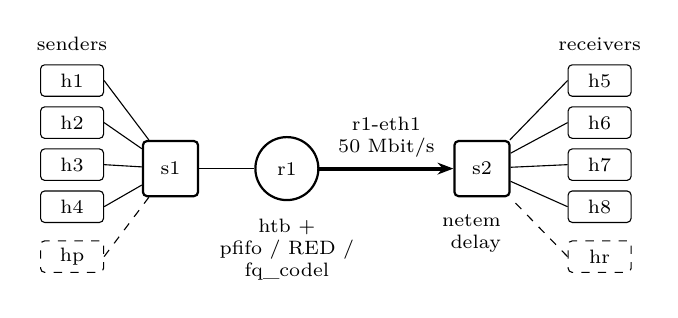
\begin{tikzpicture}[
  font=\scriptsize,
  host/.style={draw, rounded corners=1.5pt, minimum width=8mm, minimum height=4mm, inner sep=1pt},
  sw/.style={draw, thick, rounded corners=1.5pt, minimum width=7mm, minimum height=7mm},
  rt/.style={draw, thick, circle, minimum size=8mm, inner sep=0pt},
  probe/.style={host, dashed},
  node distance=1.2mm]
  \node[host] (h1) {h1};
  \node[host, below=of h1] (h2) {h2};
  \node[host, below=of h2] (h3) {h3};
  \node[host, below=of h3] (h4) {h4};
  \node[probe, below=2.2mm of h4] (hp) {hp};
  \node[sw] (s1) at ($(h1)!0.5!(hp) + (1.25,0)$) {s1};
  \node[rt, right=7mm of s1] (r1) {r1};
  \node[sw, right=17mm of r1] (s2) {s2};
  \node[host] (h5) at ($(h1) + (6.7,0)$) {h5};
  \node[host, below=of h5] (h6) {h6};
  \node[host, below=of h6] (h7) {h7};
  \node[host, below=of h7] (h8) {h8};
  \node[probe, below=2.2mm of h8] (hr) {hr};
  \foreach \h in {h1,h2,h3,h4} \draw (\h.east) -- (s1);
  \draw[dashed] (hp.east) -- (s1);
  \foreach \h in {h5,h6,h7,h8} \draw (\h.west) -- (s2);
  \draw[dashed] (hr.west) -- (s2);
  \draw (s1) -- (r1);
  \draw[-{Stealth[length=2mm]}, line width=1.4pt] (r1) -- node[above, align=center] {r1-eth1\\50 Mbit/s} (s2);
  \node[below=1mm of r1, align=center, anchor=north] {htb +\\pfifo / RED /\\fq\_codel};
  \node[above=0.5mm of h1, anchor=south] {senders};
  \node[above=0.5mm of h5, anchor=south] {receivers};
  \node[anchor=north east, align=right] at ($(s2.south east)+(0,-1mm)$) {netem\\delay};
\end{tikzpicture}
\caption{Dumbbell topology. Every flow crosses one shaped bottleneck at router port r1-eth1. The dashed probe pair hp~$\rightarrow$~hr measures RTT under load, and netem on the receiver ports of s2 sets the RTT of each path.}
\label{fig:topo}
\end{figure}

Router r1 was not part of my first design. Originally I shaped a switch port, and it failed validation: 60~Mbps of UDP arrived at the receiver as 48.7~Mbps with no loss at all, which should not be possible for a 50~Mbps link with a finite queue. The cause was that across veth pairs and Open vSwitch a packet stays charged to the socket that sent it. When the queue filled up, it pushed back on the sender and throttled it instead of dropping packets, and TCP Small Queues capped TCP in a similar way. Routing through r1 releases the packet from its socket, so the queue behaves like a real router queue. After this change the same test lost 19\% of its UDP packets, which is what a 50~Mbps link should do with 60~Mbps of offered traffic.

\section{Implementation Methodology}

\subsection{Platform}
All experiments ran in a 4-vCPU, 4~GB UTM virtual machine on an Apple M2 Mac, running Ubuntu 26.04.1 (kernel 7.0) with Mininet 2.3.0~\cite{mininet}, Open vSwitch 3.7.1, iperf 3.20~\cite{iperf3}, and Wireshark 4.6.4. I did the analysis in Python with pandas. Buffers are sized as $k \times \mathrm{BDP}$ divided into 1500~B packets, which ranges from 11 to 2,500 packets across the grid. For RED, the minimum and maximum thresholds sit at 1/6 and 1/2 of the queue limit. I turned segmentation offloads off so that the queue sees real 1514-byte frames instead of large aggregated packets.

\subsection{Automation and Metrics}
A runner script, \texttt{run.py}, expands each scenario's YAML grid into configurations, shuffles them, and interleaves their trials so that slow drift in the VM does not line up with any one configuration. Every trial builds a fresh network and first checks that the idle RTT matches the configured delay. iperf3 then runs for 60~s after a 5~s omit period that skips slow start. While it runs, \texttt{ping} samples the RTT every 0.2~s, \texttt{tc -s qdisc} records the queue backlog and drops every 0.5~s, and \texttt{ss} records each sender's cwnd and RTT every 0.1~s. For 16 configurations, tcpdump also captured the traffic for Wireshark.

All metrics cover only the time when every flow is running, which is 5--65~s, or 5--60~s in S2, where UDP stops first. Utilization is the number of bytes sent on r1-eth1 divided by $R \times t$. Queueing delay is the loaded probe RTT minus the idle median probe RTT. Jitter is iperf3's RFC~3550 estimator~\cite{rfc3550} averaged per second, and retransmissions are the sender's retransmitted bytes as a share of the bytes it sent. Each value is the mean of 5 trials (8 trials for four noisy configurations) with a 95\% confidence interval, and for most configurations that interval is under 1\% of the mean.

\subsection{Validation and Limits}
Before any experiment, I ran nine validation checks. For example, a 40~ms path measured a 40.2~ms minimum RTT, and the queue held exactly its configured limit. One thing these checks showed is that htb counts Ethernet headers against the rate. Since each 1448-byte TCP segment travels in a 1514-byte frame, TCP goodput tops out at $50 \times 1448/1514 = 47.8$~Mbps, which is why I measure utilization on the wire instead of from goodput. The VM has limits too. Its timing leaves about $\pm 4$~ms of noise in queueing delay, and its batching makes packet bursts larger than they would be on real hardware, which matters for very small buffers (Section~\ref{sec:h1}).

\section{Experimental Scenarios}

All three scenarios run Reno, CUBIC, and BBR through the same 50~Mbps bottleneck (Table~\ref{tab:scen}). No random loss is injected, so every drop happens at the bottleneck queue. S1 covers the single-flow baseline and competition between TCP flows: two or four flows with equal RTTs or with mixed RTTs from 20 to 80~ms, all using the same CCA or a CUBIC~+~BBR mix. S2 puts three TCP flows next to one UDP flow that sends at 25\% to 100\% of the link rate, to see how TCP handles traffic that never backs off. S3 varies the buffer size and the propagation delay together, first with a single flow and then with two CUBIC and two BBR flows under all three queue disciplines. In a few extra runs BBR (S1) or UDP (S2) starts late, so that the captures show the moment a new flow joins.

\begin{table*}[t]
\caption{Experimental Scenarios (Defaults: 40~ms RTT, 1\x{} BDP Buffer, pfifo). Trials Include 3 Late-BBR (S1) and 2 Late-UDP (S2) Runs}
\label{tab:scen}
\centering
\begin{tabular}{@{}L{3.6cm}L{10.2cm}cc@{}}
\toprule
Scenario & Grid & Configs & Trials \\
\midrule
S1: Competing TCP flows & 1 flow per CCA; 2 or 4 flows \x{} equal or mixed RTTs (20--80~ms) \x{} Reno, CUBIC, BBR, or CUBIC~+~BBR \x{} pfifo, fq\_codel & 35 & 178 \\
S2: TCP + UDP & 3 TCP + 1 UDP flow at 25, 50, 75, 100\% of $R$ \x{} CCA \x{} pfifo, fq\_codel & 24 & 131 \\
S3: Buffer and delay & 1 flow: 0.25\x, 1\x, 4\x{} BDP \x{} RTT 10, 50, 150~ms \x{} CCA; 2 CUBIC + 2 BBR at 50~ms: buffer \x{} pfifo, RED, fq\_codel & 36 & 183 \\
\midrule
Total & & 95 & 492 \\
\bottomrule
\end{tabular}
\end{table*}

\section{Results}

\subsection{S1: Competing Flows}
Any single flow on its own filled the link. Utilization was 99.98\% for Reno, 99.97\% for CUBIC, and 97.5\% for BBR. The difference was in delay, where CUBIC kept 27.9~ms of queueing delay and Reno 22.6~ms, while BBR added only 0.8~ms. Flows using the same CCA with equal RTTs shared fairly, with Jain's index of about 0.95 or higher. Mixing CCAs on pfifo was a different story. CUBIC kept only 10.6\% of the throughput against one BBR flow, 1.9--3.3\% in a 2~+~2 mix, and about 5~Mbps when BBR joined late. With mixed RTTs (Fig.~\ref{fig:fair}), Reno gave its 20~ms flow 37.6\% of the link in the four-flow case (Jain 0.88), while CUBIC was fairer at 0.95. BBR reversed the bias. Its 80~ms flow took 39.4\% and its 20~ms flow only 6.7\% (Jain 0.74). Two or four BBR flows on pfifo also retransmitted 3.6--10.6\% of their bytes, compared with under 0.06\% for Reno and CUBIC.

\begin{figure*}[t]
\centering
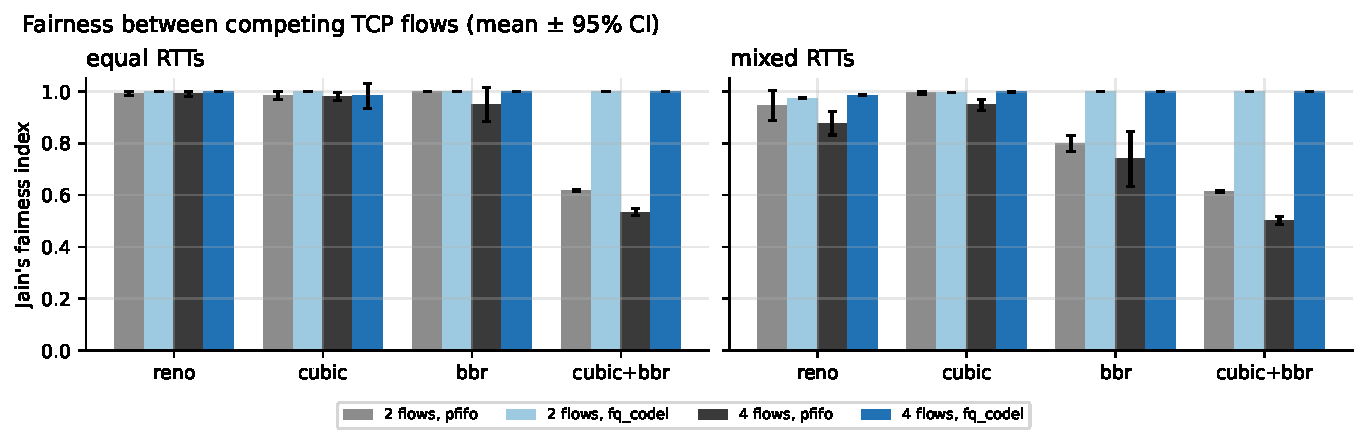
\includegraphics[width=0.92\textwidth]{figs/F2_s1_fairness.pdf}
\caption{Jain's fairness index in S1 (mean $\pm$ 95\% CI). The CUBIC + BBR mix on pfifo is the lowest, while fq\_codel stays between 0.97 and 1.00 everywhere.}
\label{fig:fair}
\end{figure*}

\subsection{S2: TCP and UDP}
On pfifo, the three CUBIC flows together got 35.5, 23.1, 10.7, and 0.05~Mbps as UDP's offered load rose from 25\% to 100\% of $R$, and Reno and BBR were within 0.9~Mbps of these numbers. fq\_codel held TCP at 33--35~Mbps at every load by dropping UDP's excess instead, so UDP loss reached 75\%. The trade-off was jitter. At 75--100\% load, UDP jitter under fq\_codel rose to 0.6--0.8~ms, compared with at most 0.11~ms on pfifo (Fig.~\ref{fig:s2}).

\begin{figure*}[t]
\centering
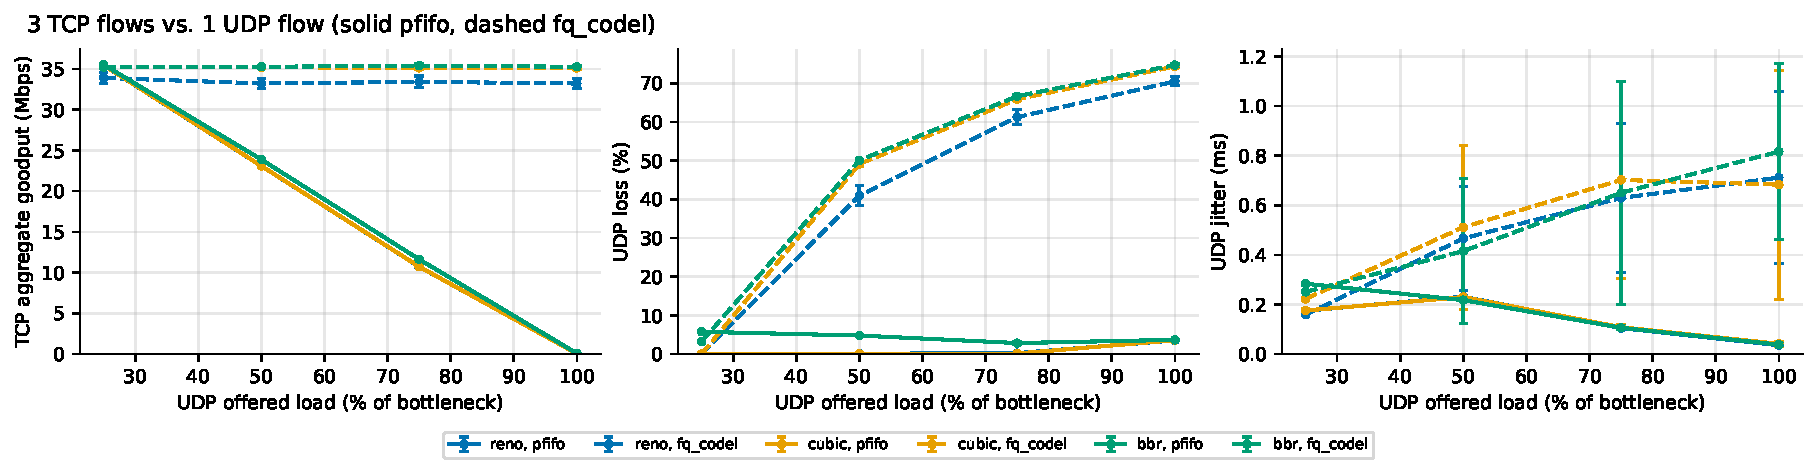
\includegraphics[width=0.98\textwidth]{figs/F4_s2_tcp_vs_udp.pdf}
\caption{TCP goodput, UDP loss, and UDP jitter versus UDP offered load in S2 (solid pfifo, dashed fq\_codel). Under fq\_codel, TCP keeps roughly three quarters of the link no matter how hard UDP pushes.}
\label{fig:s2}
\end{figure*}

\subsection{S3: Buffers and RTT}
With 1\x{} BDP of buffer or more, every CCA stayed above 96\% utilization. At 0.25\x{} BDP, Reno dropped to 82--87\%, while CUBIC kept 98\% and BBR 95--97\%. The one exception was the 11-packet buffer at 10~ms, where Reno and CUBIC both fell to 23\% (Fig.~\ref{fig:util}). On pfifo, CUBIC's share against BBR went from 1.4\% to 1.8\% to 58.9\% as the buffer grew from 0.25\x{} to 4\x{} BDP. RED kept CUBIC at about 2\% regardless of the buffer, and fq\_codel kept it at about 48\% (Fig.~\ref{fig:share}).

Deep buffers also showed the delay cost of loss-based CCAs. At 4\x{} BDP, a single CUBIC flow added 34.5, 162, and 494~ms of queueing delay at RTTs of 10, 50, and 150~ms. Reno added 28, 127, and 245~ms, and BBR stayed under 3~ms. With the four mixed flows at 4\x{} BDP, queueing delay was 164~ms on pfifo, 48~ms on RED, and about 0 on fq\_codel.

\begin{figure*}[t]
\centering
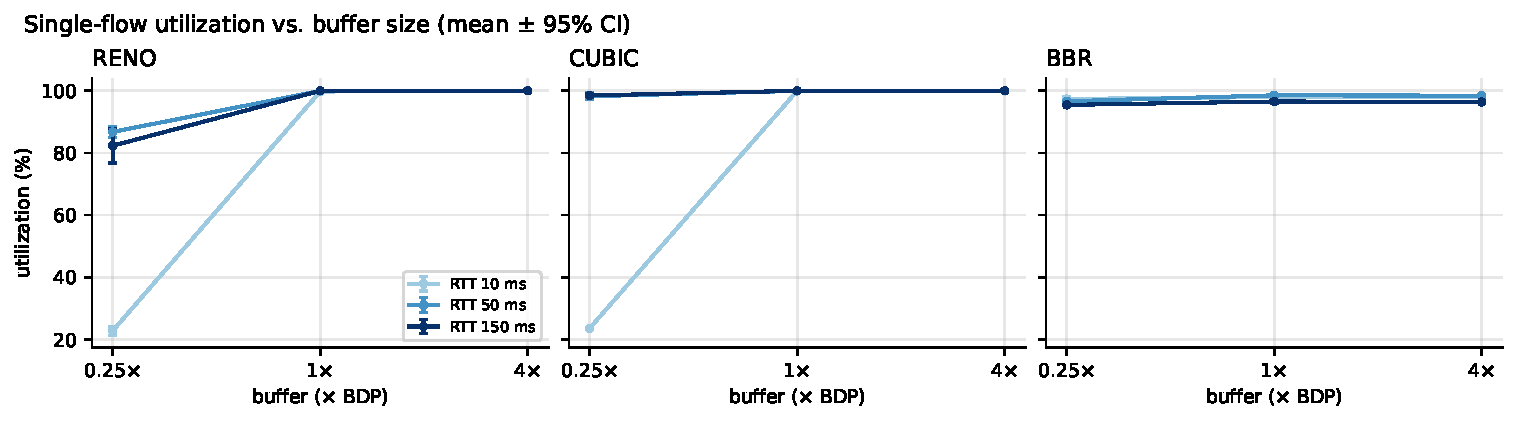
\includegraphics[width=0.92\textwidth]{figs/F5_s3_utilization_vs_buffer.pdf}
\caption{Single-flow utilization versus buffer size in S3. Only shallow buffers cost throughput, and only for the loss-based CCAs.}
\label{fig:util}
\end{figure*}

\begin{figure*}[t]
\centering
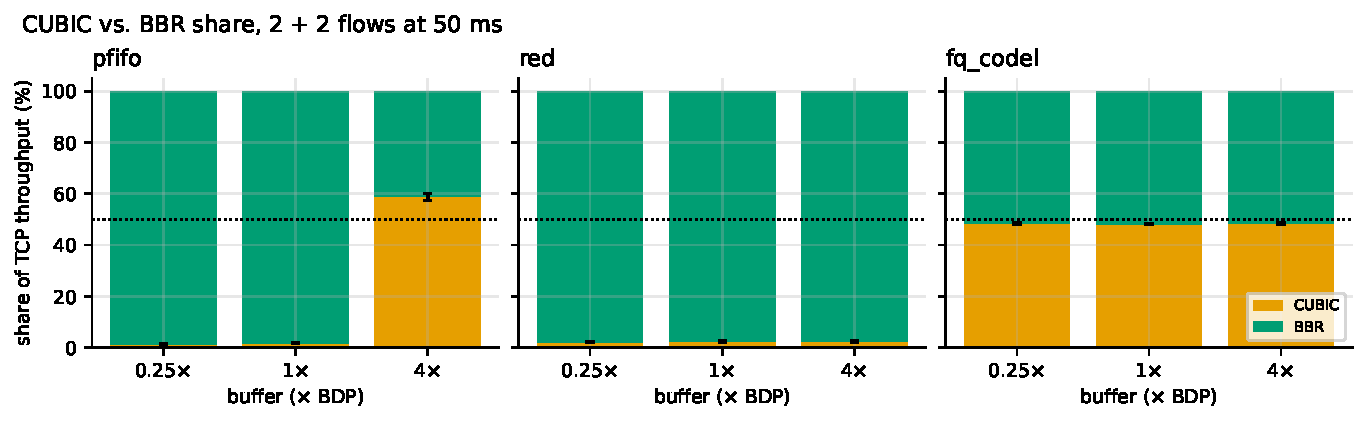
\includegraphics[width=0.92\textwidth]{figs/F6_s3_cubic_vs_bbr.pdf}
\caption{CUBIC's share of TCP throughput against BBR (2 + 2 flows, 50~ms). On pfifo it follows the buffer depth, RED leaves CUBIC near 2\%, and fq\_codel evens it out.}
\label{fig:share}
\end{figure*}

\section{Analysis and Discussion}
\label{sec:analysis}

Most of the results come down to two properties: how each sender responds to loss, and whether the queue keeps flows isolated from each other. Table~\ref{tab:hyp} summarizes how each hypothesis from my proposal held up, and the rest of this section explains why.

\begin{table}[t]
\caption{Proposal Hypotheses and What the Data Showed}
\label{tab:hyp}
\centering
\renewcommand{\arraystretch}{1.25}
\begin{tabular}{@{}L{4.6cm}L{3.7cm}@{}}
\toprule
Hypothesis & Verdict \\
\midrule
H1: $\geq$90\% utilization at $\geq$1\x{} BDP; Reno 85--90\% at 0.25\x & Partly, plus an 11-packet collapse \\
H2: Reno favors short RTTs more than CUBIC & Supported; BBR reverses it \\
H3: BBR wins shallow buffers, CUBIC deep ones & Supported on pfifo, not RED \\
H4: Line-rate UDP starves TCP; fq\_codel fixes it & Supported \\
H5: A deep FIFO adds about its drain time & CUBIC yes; Reno partly \\
\bottomrule
\end{tabular}
\end{table}

\subsection{H1: Utilization}
\label{sec:h1}
The link goes idle whenever cwnd falls below one BDP, since the sender then cannot keep enough data in flight. With $b$ BDPs of buffer, a loss-based flow's cwnd peaks at $(1+b)$~BDP right before the buffer overflows. Reno then halves and regrows linearly, which for $b = 0.25$ means cwnd drops to 0.625~BDP and spends part of every cycle below 1~BDP. This simple model predicts 89\% utilization, and I measured 86.7\% at 50~ms. The Wireshark capture in Fig.~\ref{fig:inflight} shows this cycle directly. Bytes in flight dip to about 186~KB after each loss, well below the 312~KB BDP, and then climb back at one segment per RTT. Each cycle takes about 7~s, since Reno needs about 130 RTTs to grow back. CUBIC's 0.7\x{} cut keeps cwnd at 0.875~BDP or above, which predicts 98\% (measured 98.2\%). At 150~ms Reno needs more than a minute to regrow, so most trials never finish a single cycle after startup. BBR does not react to loss, and its 2--4\% shortfall comes mostly from ProbeRTT draining the queue every 10~s.

\begin{figure*}[t]
\centering
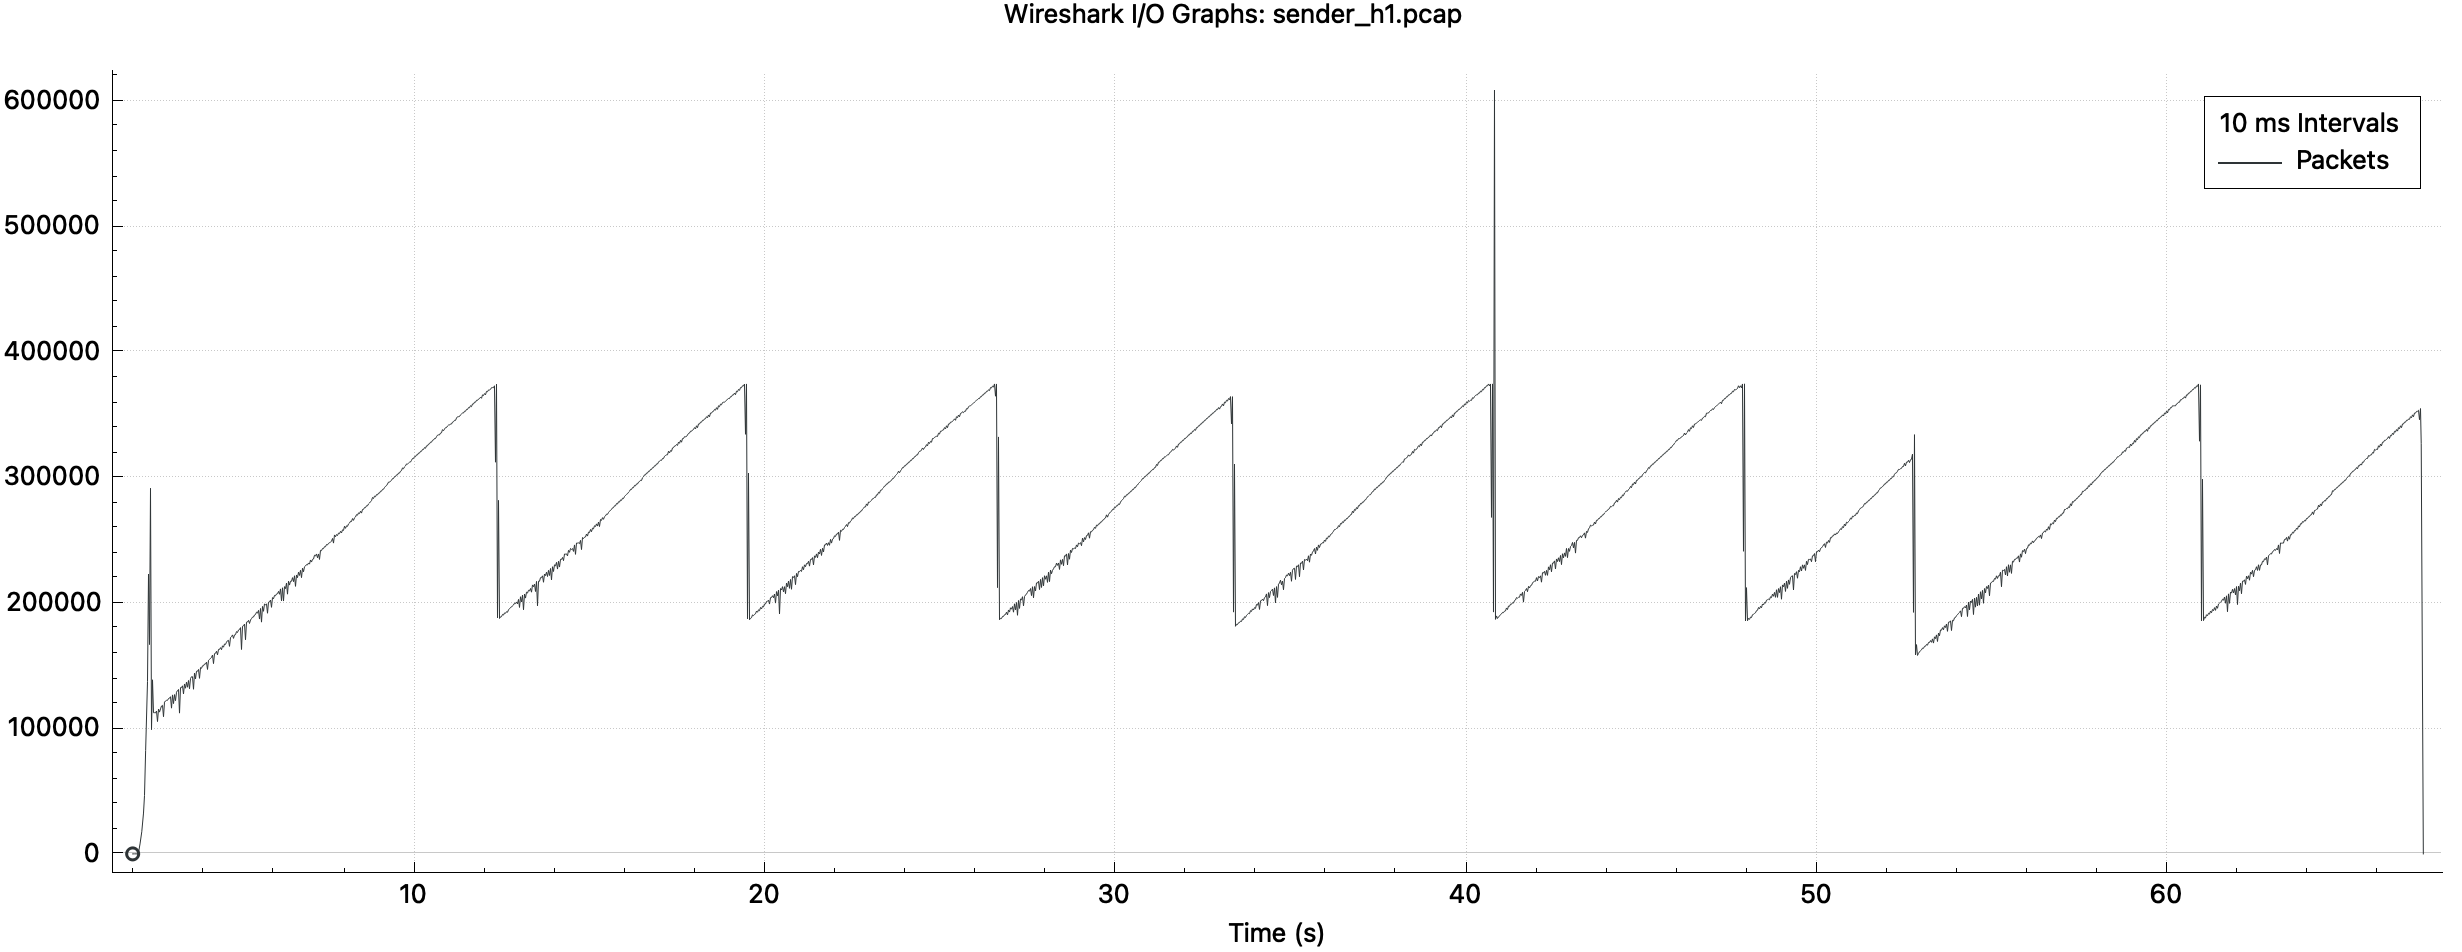
\includegraphics[width=0.78\textwidth]{figs/capture_reno_inflight.png}
\caption{Wireshark I/O graph of bytes in flight for one Reno flow with a 0.25\x{} BDP buffer at 50~ms RTT (S3, sender capture, 10~ms bins). Each loss halves the window to about 186~KB, below the 312~KB BDP, so the link sits partly idle until the window grows back.}
\label{fig:inflight}
\end{figure*}

The 11-packet collapse was not something I predicted. In this case, unpaced bursts from Reno and CUBIC overflow the tiny queue with about 1,000 drops per trial, and the repeated losses pin cwnd near 11 packets against a 42-packet BDP. Paced BBR lost even more, about 9,500 packets per trial, and still kept 97\% utilization since it does not cut its rate on loss. This lines up with earlier work showing that tiny buffers only work with smooth traffic~\cite{enachescu}, and VM batching most likely makes the effect worse than it would be on real hardware.

\subsection{H2 and H3: Sharing Between Flows}
After a loss that hits both flows, Reno's 20~ms flow regrows about twice as fast as its 80~ms flow, because their effective RTTs including the queue are 49 and 109~ms. This is why short-RTT Reno flows win. CUBIC's time-based growth narrows the gap, which matches its higher Jain index. BBR flips the bias for a different reason. It caps its data in flight using its own minimum RTT, so a flow with a longer RTT is allowed more data in flight and ends up holding more of the FIFO~\cite{hock,ware}.

The same idea explains CUBIC against BBR. In shallow buffers, BBR keeps sending through the losses it causes, while CUBIC backs off on every one of them. At 4\x{} BDP the roles flip. CUBIC can fill the large queue before any loss happens, but BBR's in-flight cap does not grow with the queueing delay, so CUBIC wins with 58.9\%. RED drops packets from both, but only CUBIC responds to those drops, so BBR stays on top at every buffer size. Under fq\_codel's round-robin, each flow gets its turn no matter how large its window is, so window size stops mattering.

\subsection{H4: TCP Beside UDP}
In a shared queue, every drop makes a TCP flow halve its rate, but UDP keeps sending at the same rate no matter what. This means TCP ends up with whatever UDP leaves behind. With 1242-byte UDP frames on the wire, this predicts 35.4, 23.1, 10.7, and 0~Mbps for TCP, which is within 0.1~Mbps of what I measured for CUBIC and Reno. At 100\% load, 3.4\% of UDP's frames cannot fit on the link, which matches its measured 3.6\% loss. Fig.~\ref{fig:udp} shows what this looks like on the wire. When UDP joins, TCP collapses within 0.3~s, and 21\% of its remaining packets are retransmissions. TCP only recovers once UDP stops.

\begin{figure*}[t]
\centering
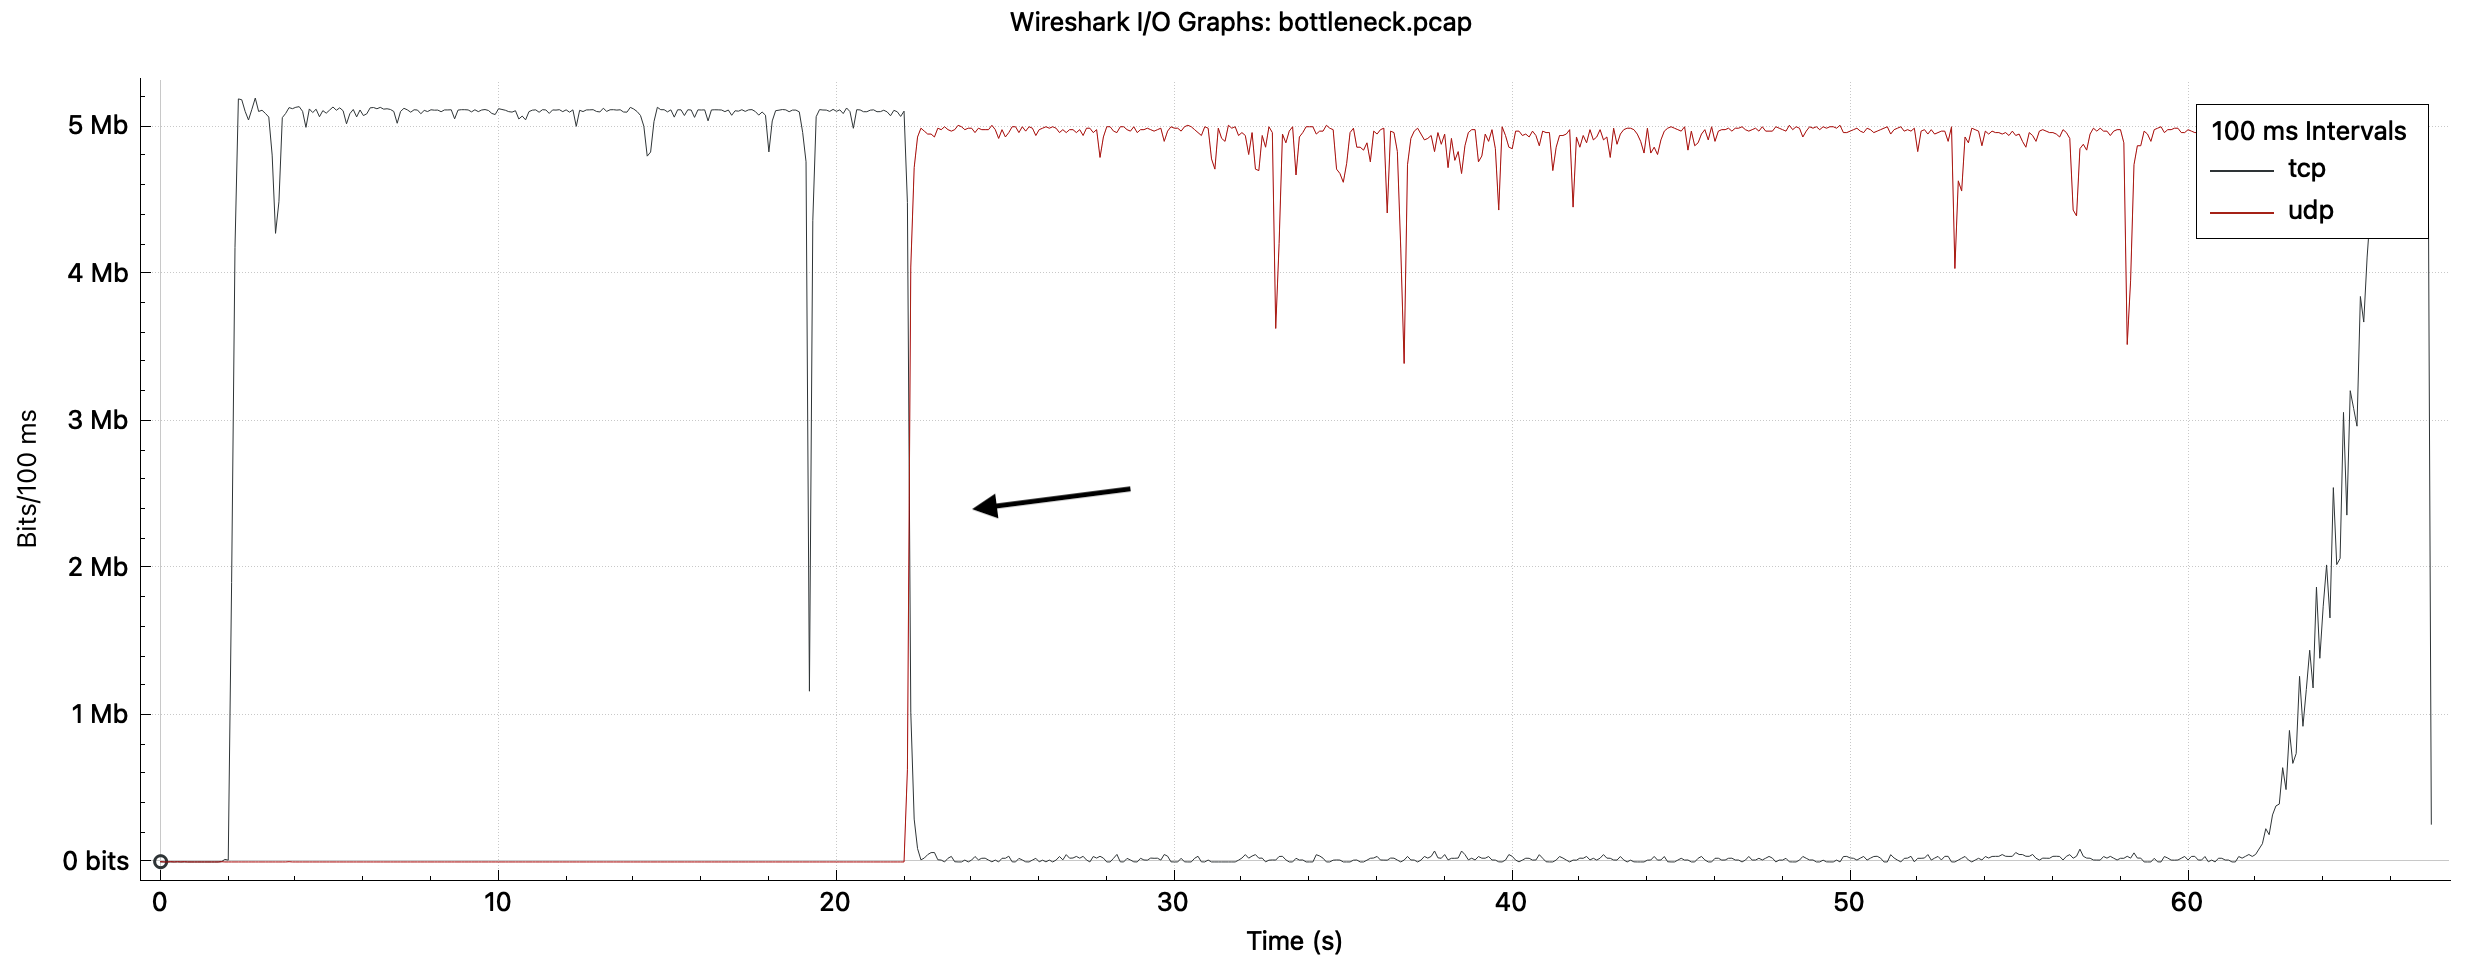
\includegraphics[width=0.78\textwidth]{figs/capture_late_udp.png}
\caption{Wireshark I/O graph of the bottleneck capture for 3 CUBIC flows and UDP at 100\% load on pfifo, with UDP starting late (trial 1, 100~ms bins, black TCP and red UDP). TCP collapses when UDP joins at 22~s capture time (arrow) and recovers only after UDP stops.}
\label{fig:udp}
\end{figure*}

fq\_codel avoids this by giving each of the four flows a quarter of the link. The cost is that UDP's packets are now interleaved with TCP bursts, which raises its jitter. Switching the TCP senders to BBR does not help either. At only 25\% UDP load, BBR caused 5.8\% UDP loss compared with 0.06\% under CUBIC. My best explanation is that BBR's probing kept the FIFO full, although BBR still caused 3.2\% UDP loss under fq\_codel, so the queue is probably not the whole story.

\subsection{H5: Queueing Delay}
A 4\x{} BDP buffer takes 4\x{} RTT to drain, which is 40, 200, and 600~ms at the three RTTs. CUBIC's 0.7\x{} cut leaves most of the buffer full, so its queue stayed 80--86\% full on average, and the captured RTT on a 50~ms path ranged from 175 to 250~ms. Reno cycling between 2.5 and 5~BDP should keep the buffer 69\% full on average, which matches the 64--71\% I measured at 10 and 50~ms. At 150~ms, though, Reno never fully regrows within the 60~s trial, so it only reached 41\%. A single BBR flow keeps about one BDP in flight and CoDel drops packets after 5~ms of waiting, so neither one builds a standing queue. Several BBR flows on pfifo are a different case, since together they kept 37--40~ms of queue in S1.

\subsection{Testbed Lessons}
Besides the router fix in Section~\ref{sec:arch}, two measurement choices turned out to matter. First, utilization has to be counted on the wire, since goodput hides the header overhead. Second, metrics have to cover only the time when all flows overlap. My first S2 analysis did not do this. The UDP client ran from 0 to 60~s while TCP ran until 65~s, so the TCP numbers included 5~s with no UDP at all. Because of this, TCP next to line-rate UDP appeared to get 2.2~Mbps, which all arrived after UDP had stopped.

\section{Design Recommendations}

Ultimately, changing the bottleneck queue helps more than changing any CCA. The CCA choice only matters where a FIFO has to stay, for example on equipment the operator cannot reconfigure. Table~\ref{tab:rec} lists what I would deploy for each condition, along with the evidence behind it. These come from a single 50~Mbps bottleneck in a VM, with BBRv1 and 60~s flows, so they should be treated as a starting point and not as a rule for every network.

\begin{table*}[t]
\caption{Recommendations for One 50~Mbps Bottleneck (BBRv1, 60~s Flows, in a VM)}
\label{tab:rec}
\centering
\begin{tabular}{@{}L{4.6cm}L{5.4cm}L{6.0cm}@{}}
\toprule
Condition & Recommendation & Evidence \\
\midrule
Operator controls the bottleneck & fq\_codel, any CCA & Delay $\sim$0~ms; Jain $\geq$0.97 \\
Unresponsive UDP & fq\_codel; no CCA helps & TCP $<$0.1~Mbps on pfifo \\
Mixed CCAs or RTTs on a FIFO & fq\_codel, not RED & CUBIC 1.4--10.6\% vs.\ BBR \\
Deep FIFO ($\geq$4\x{} BDP) & fq\_codel, $\sim$1\x{} BDP, or BBR & CUBIC +494~ms; BBR $<$3~ms \\
$\sim$1\x{} BDP FIFO, one CCA & BBR for latency, CUBIC for throughput & BBR 0--3~ms; CUBIC $\sim$100\% \\
Shallow FIFO ($\leq$0.25\x{} BDP) & BBR, or CUBIC at RTT $\geq$50~ms & Reno 82--87\%; 23\% at 10~ms \\
\bottomrule
\end{tabular}\\[3pt]
{\footnotesize Under fq\_codel, Reno loses about 5\% of its throughput.}
\end{table*}

\section{Conclusion}

Across 492 trials, the bottleneck queue shaped fairness and delay more than the senders' CCA did. On a FIFO, BBR and UDP take bandwidth from flows that back off on loss, and loss-based senders turn deep buffers into hundreds of milliseconds of delay. fq\_codel removed all of these effects at the cost of under 1~ms of UDP jitter and up to 5.5\% of Reno's throughput. If a FIFO has to stay, BBR is the better fit for low latency and tiny buffers as long as every sender uses it, while CUBIC is the safer choice for long or mixed RTTs. As of right now these conclusions only cover one bottleneck. Future work could extend them to a two-bottleneck parking-lot topology, BBRv3, and real hardware without VM batching, where the small-buffer results in particular could turn out quite different.

\begin{thebibliography}{99}

\bibitem{gettys}
J.~Gettys and K.~Nichols, ``Bufferbloat: Dark buffers in the Internet,'' \emph{ACM Queue}, 2011.

\bibitem{jacobson}
V.~Jacobson, ``Congestion avoidance and control,'' in \emph{Proc. ACM SIGCOMM}, 1988.

\bibitem{rfc5681}
M.~Allman, V.~Paxson, and E.~Blanton, ``TCP congestion control,'' IETF RFC 5681, Sep. 2009. [Online]. Available: \url{https://www.rfc-editor.org/rfc/rfc5681}

\bibitem{cubic}
S.~Ha, I.~Rhee, and L.~Xu, ``CUBIC: A new TCP-friendly high-speed TCP variant,'' \emph{ACM SIGOPS Operating Systems Review}, 2008.

\bibitem{bbr}
N.~Cardwell \emph{et al.}, ``BBR: Congestion-based congestion control,'' \emph{ACM Queue}, 2016.

\bibitem{red}
S.~Floyd and V.~Jacobson, ``Random early detection gateways for congestion avoidance,'' \emph{IEEE/ACM Trans. Netw.}, 1993.

\bibitem{rfc8290}
T.~H{\o}iland-J{\o}rgensen \emph{et al.}, ``The flow queue CoDel packet scheduler and active queue management algorithm,'' IETF RFC 8290, Jan. 2018. [Online]. Available: \url{https://www.rfc-editor.org/rfc/rfc8290}

\bibitem{codel}
K.~Nichols and V.~Jacobson, ``Controlling queue delay,'' \emph{ACM Queue}, 2012.

\bibitem{appenzeller}
G.~Appenzeller, I.~Keslassy, and N.~McKeown, ``Sizing router buffers,'' in \emph{Proc. ACM SIGCOMM}, 2004.

\bibitem{jain}
R.~Jain, D.~Chiu, and W.~Hawe, ``A quantitative measure of fairness and discrimination for resource allocation in shared computer systems,'' Digital Equipment Corp., Tech. Rep. DEC-TR-301, 1984.

\bibitem{mininet}
N.~Handigol \emph{et al.}, ``Reproducible network experiments using container-based emulation,'' in \emph{Proc. ACM CoNEXT}, 2012.

\bibitem{iperf3}
ESnet, ``iperf3.'' [Online]. Available: \url{https://github.com/esnet/iperf}

\bibitem{rfc3550}
H.~Schulzrinne \emph{et al.}, ``RTP: A transport protocol for real-time applications,'' IETF RFC 3550, Jul. 2003. [Online]. Available: \url{https://www.rfc-editor.org/rfc/rfc3550}

\bibitem{enachescu}
M.~Enachescu \emph{et al.}, ``Routers with very small buffers,'' in \emph{Proc. IEEE INFOCOM}, 2006.

\bibitem{hock}
M.~Hock, R.~Bless, and M.~Zitterbart, ``Experimental evaluation of BBR congestion control,'' in \emph{Proc. IEEE ICNP}, 2017.

\bibitem{ware}
R.~Ware \emph{et al.}, ``Modeling BBR's interactions with loss-based congestion control,'' in \emph{Proc. ACM IMC}, 2019.

\end{thebibliography}

\end{document}
